% Asset ID: A21DifferentiationTikZ-004
% Source: Chapter 9 second derivative evidence
% Related lesson section: Second derivative and inflection
% Purpose: Show concavity, convexity and point of inflection.
\documentclass[tikz,border=8pt]{standalone}
\usepackage{amsmath}
\usepackage{pgfplots}
\pgfplotsset{compat=1.18}
\begin{document}
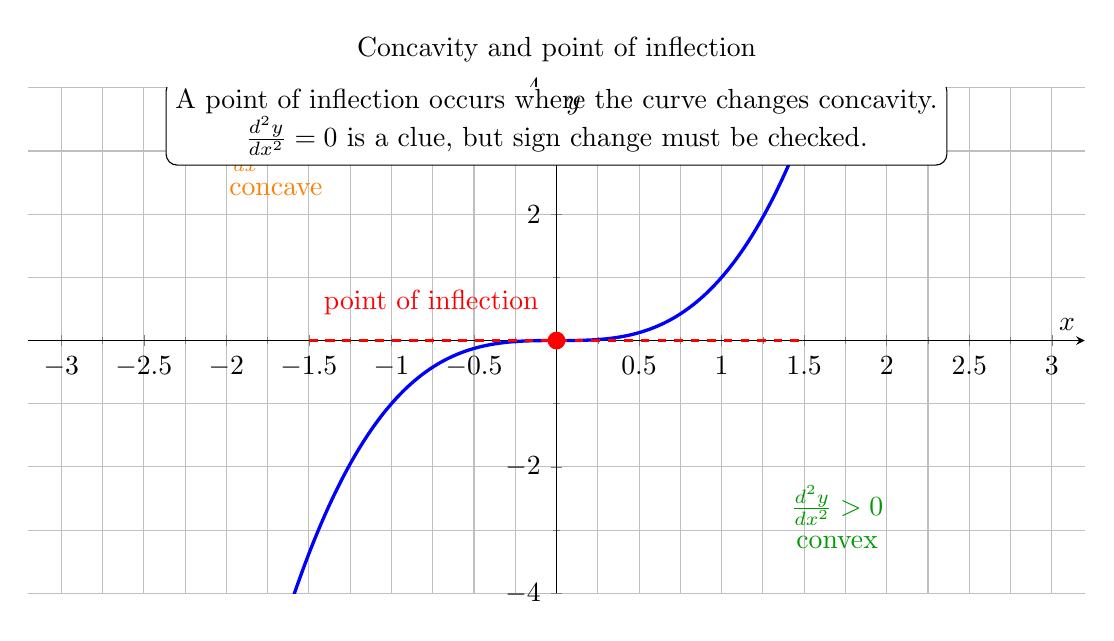
\begin{tikzpicture}
\begin{axis}[width=15cm,height=8cm,axis lines=middle,xmin=-3.2,xmax=3.2,ymin=-4,ymax=4,xlabel={$x$},ylabel={$y$},title={Concavity and point of inflection},samples=300,domain=-2.6:2.6,grid=both,minor tick num=1]
\addplot[very thick, blue] {x^3};
\addplot[only marks, mark=*, mark size=3pt, red] coordinates {(0,0)};
\node[red, anchor=south east] at (axis cs:-0.05,0.25) {point of inflection};
\node[orange, align=center] at (axis cs:-1.7,2.8) {\(\frac{d^2y}{dx^2}<0\)\\concave};
\node[green!60!black, align=center] at (axis cs:1.7,-2.8) {\(\frac{d^2y}{dx^2}>0\)\\convex};
\addplot[red, thick, dashed, domain=-1.5:1.5] {0};
\node[draw, rounded corners, fill=white, align=center] at (axis cs:0,3.45) {A point of inflection occurs where the curve changes concavity.\\\(\frac{d^2y}{dx^2}=0\) is a clue, but sign change must be checked.};
\end{axis}
\end{tikzpicture}
\end{document}
